\chapter{Architecture and Design }

\section{Introduction }
In this chapter, we will embark on a crucial part of software development that bridges the gap between specification and implementation. This entails the design of the application. We will first present the general design of our application, followed by the detailed design including static views through class diagrams and dynamic views through sequence diagrams. 

\section{Architecture  }

• \textbf{MVC Architecture} 

The Model-View-Controller or MVC is a software architectural pattern intended for graphical interfaces, launched in 1978 and widely popular for web applications. The pattern consists of three types of modules with three different responsibilities: models, views, and controllers.

\begin{itemize}
    \item A model (Model) contains the data to display.
    \item A view (View) contains the presentation of the graphical interface.
    \item A controller (Controller) contains the logic concerning the actions performed by the user.
\end{itemize}
 
\begin{figure}[H]
   \centering
    %\includegraphics[scale=0.5]{images/trasfvs.jpg}
    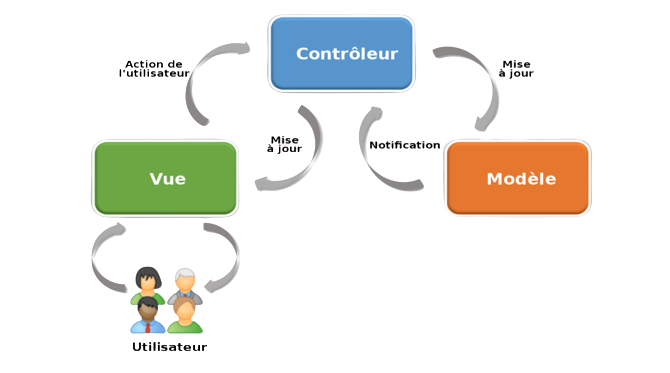
\includegraphics[width=15cm,height=8cm]{images/MVC.png}
    \caption{MVC Architecture} 
    \label{MVC Architecture}
\end{figure}

\section{Application mockups   }

"Authentication Mockup" To access the application, the user must either authenticate or sign up. 

\begin{figure}[H]
   \centering
    %\includegraphics[scale=0.5]{images/trasfvs.jpg}
    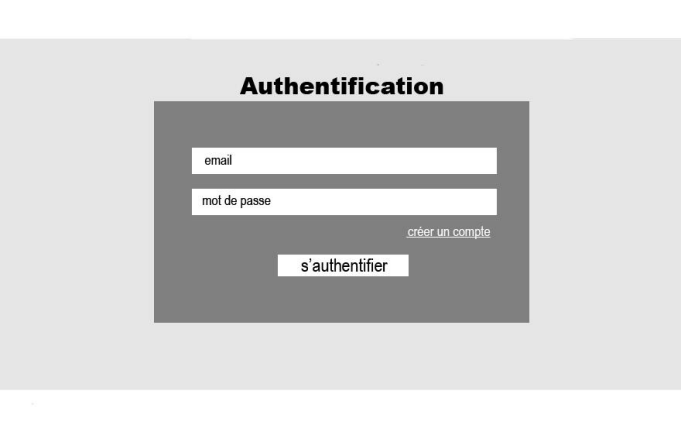
\includegraphics[width=15cm,height=8cm]{images/maqauth.png}
    \caption{Authentication Mockup} 
    \label{Authentication Mockup}
\end{figure}

"Sign Up Mockup" To access the application, the user must create an account. 

\begin{figure}[H]
   \centering
    %\includegraphics[scale=0.5]{images/trasfvs.jpg}
    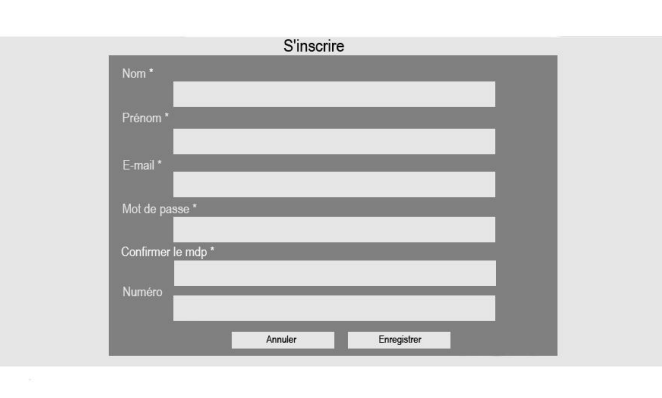
\includegraphics[width=15cm,height=8cm]{images/maqinsc.png}
    \caption{Sign Up Mockup} 
    \label{Sign Up Mockup}
\end{figure}




\section{Detailed design   }
\subsection{Class diagram  }

The class diagram is a static representation of the elements that make up a system and their relationships. The figure includes the main classes of our application and their associations. 

\begin{figure}[H]
   \centering
    %\includegraphics[scale=0.5]{images/trasfvs.jpg}
    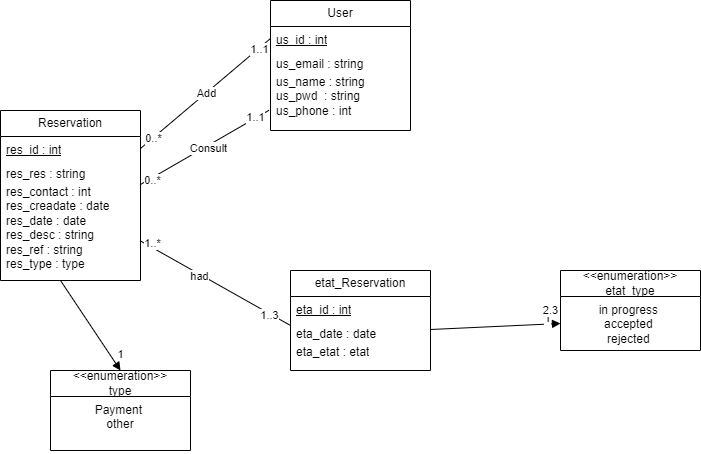
\includegraphics[width=15cm,height=8cm]{images/class.drawio.png}
    \caption{Class diagram} 
    \label{class diagram}
\end{figure}

\subsection{Sequence diagrams   }
The sequence diagrams provide a dynamic view of the interaction between the actor and the system. In this section, we represent the sequence diagrams related to some usage scenarios of our system .
    \item \textbf{Sequence diagram: Authentication }
\begin{figure}[H]
   \centering
    %\includegraphics[scale=0.5]{images/trasfvs.jpg}
    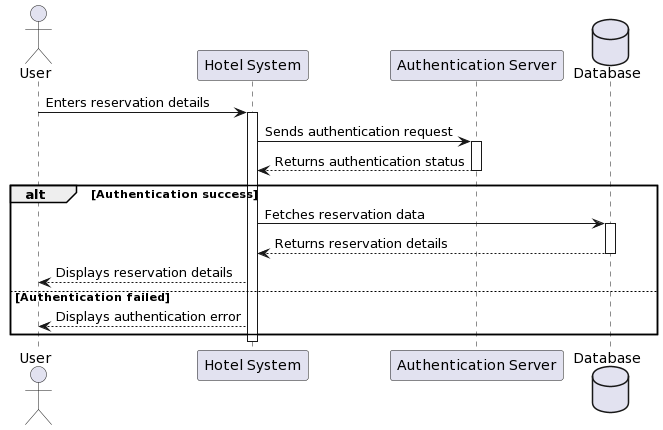
\includegraphics[width=15cm,height=8cm]{images/seq.png}
    \caption{Sequence diagram: Authentication } 
    \label{Sequence diagram: Authentication }
\end{figure}
\item \textbf{Sequence diagram: Manage reservation}

\begin{figure}[H]
   \centering
    %\includegraphics[scale=0.5]{images/trasfvs.jpg}
    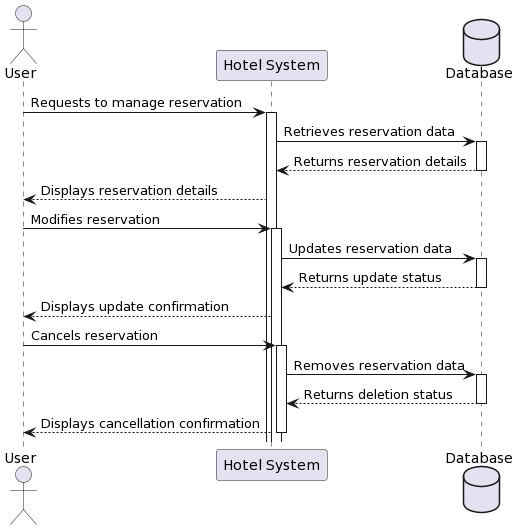
\includegraphics[width=15cm,height=8cm]{images/seq2.png}
    \caption{Sequence diagram: Manage reservation } 
    \label{Sequence diagram: Manage reservation  }
\end{figure}

\subsection{Activity diagram    }

This activity diagram provides a view of the behavior of a system by describing the sequence of actions in a process. 
\begin{figure}[H]
   \centering
    %\includegraphics[scale=0.5]{images/trasfvs.jpg}
    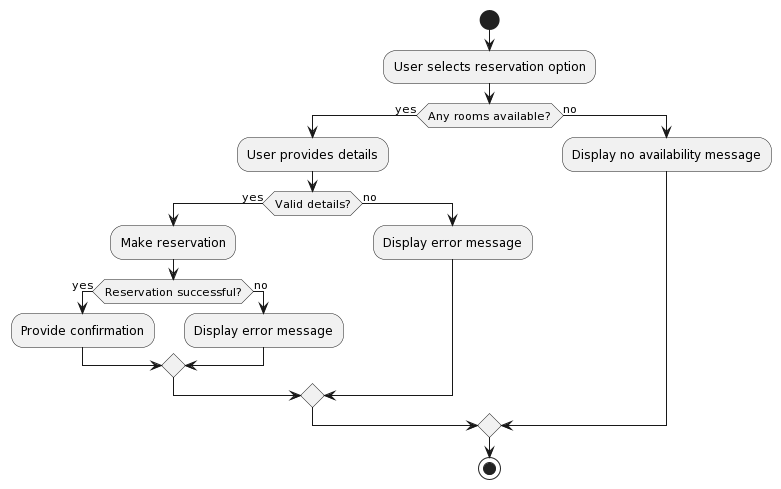
\includegraphics[width=15cm,height=8cm]{images/act.png}
    \caption{Activity diagram : manage reservation } 
    \label{activity diagram : manage reservation }
\end{figure}

\section{Conclusion }
Through this chapter, we have established the design of our application. Firstly, we began by outlining the architecture of our work, then we presented the class diagram that we deemed necessary to understand the functioning of our application. With the design of our module established, we now move on to the implementation phase. 